\chapter{Background}\label{Ch:Background}
In this chapter, we introduce the models that we study in this paper, both ordered and disordered systems. For disordered systems, we will explain how we introduce randomness into the system. 



\section{Model 1}\label{model:model1}
\subsection{model 1a}

The model we are studying is represented by the one-dimensional time-independent Schrodinger equation: 
\begin{equation} \label{eq:2.1}
-\frac{d^2\psi}{dx^2}+V(x)\psi=E\psi
\end{equation}
where the potential consist of non-overlapping atomic potential similar to the Kronig Penny model. But we use finite negative square well potential instead of delta potential at each atom site (See the figure below).

Also, for this model we impose zero boundary conditions for the wave function. This means the potential is positive infinity at two ends. 

\begin{figure}[h]
\centering
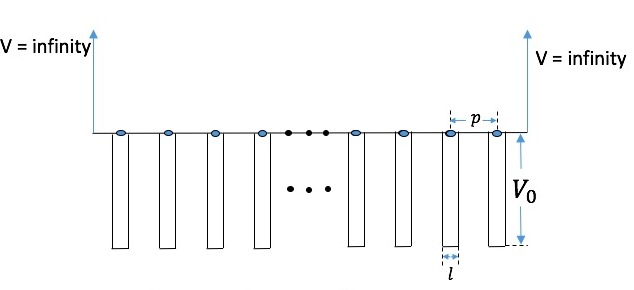
\includegraphics[scale=0.75]{Graphics/square_potential_problem.jpeg}
\caption{Model1a, $p$, $l$, $V_0$ denotes atom spacing, square well width, and potential height respectively}
\label{fig:net}
\end{figure}

\newpage
\subsection{model 1b}
Model 1b is derived from model 1a by introducing some randomness to atomic spacing to a chain of atoms. With potential height($V_0$) and well width($l$) fixed, the atomic spacing between any two atoms now takes two values from ${\{p_1,p_2\}}$ with probability ${\{P(p_1),P(p_2)\}}$. The boundary conditions are the same as in model 1a.
\subsection{model 1c}
In model 1c, randomness is introduced to the potential well at each atom site. This time, both atomic spacing and potential well width  are  fixed, but the potential height at each atom site takes a value from $\{V_1,V_2\}$ with probability $\{P(V_1),P(V_2)\}$. Again, the same boundary condition as in model 1a applies to model 1c. 

\section{Model 2}\label{bloch theorem}
In this model we study a chain of atoms with non-overlapping negative square well potential under periodic boundary conditions. (See figure below).
\begin{figure}[h]
\centering
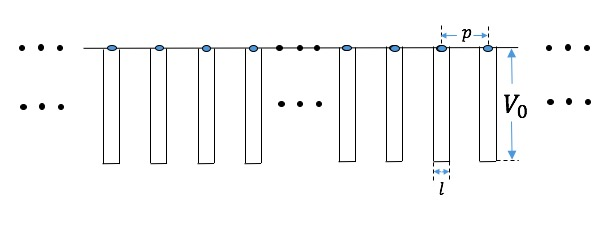
\includegraphics[scale=0.75]{Graphics/kp_bandgap.jpeg}
\caption{Model2}
\label{fig:net}
\end{figure}
The corresponding time-independent Schrodinger equation that governs that system is the same as equation \ref{eq:2.1} but with the potential being periodic with a period $p$, i.e. $V(x) = V(x+p)$ in this case. 
If we consider a sample of N atoms, due to the periodicity, we may impose the Von Karman condition\cite{BoundaryCondition} at the macroscopic boundary,i.e. $\psi(x+Np) = \psi(x)$. 
By use of Bloch theorem \cite{BlochTheorem}, we know that the solution would be of the form $$\psi_k(x) = e^{i{\alpha_k}x}u_k(x),$$ with $u_k(0) = u_k(p)$,
and $\alpha_k$ taking values (Note that $\alpha_k$ is called the wave vector)
$$\alpha_k = \frac{x\pi k}{Np}, \quad k = -\frac{Np}{2},...,\frac{Np}{2}. $$
After substituting it into equation \ref{eq:2.1}, we can get
\begin{equation}\label{eq:2.2bloch}
-\frac{1}{2}(\frac{d}{dx}+i\alpha_k)^2u_k+V(x)u_k = Eu_k
\end{equation}

With the above equation, for each wave vector, we can solve the Schr\"{o}dinger equation and get the corresponding eigenvalues. If we plot the eigenvalues against wave wave vectors. We can obtain a band structure for this one-dimensional periodic system, from which we can determine the band gap, which is the difference of the smallest eigenvalue in the second band and the largest eigenvalue in the first band.

\section{Model 3}
In this model, we consider a chain of $N+1$ atoms connected by harmonic strings, meaning that the interaction between the nearest neighboring atoms obey Hooke's law. The system is shown in the following graph. 
\begin{figure}[h]
\centering
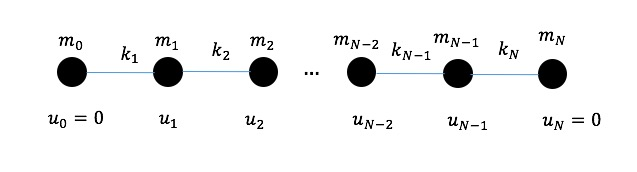
\includegraphics[scale=0.75]{Graphics/harmonicChain.jpeg}
\caption{Model 3:Harmonic chain model}
\label{fig:net}
\end{figure}
As shown in this graph,  $k_n$ is the elastic constant of the harmonic string between the $(n-1)$th and $n$th atom. $u_n$ and $m_n$ are respectively the displacement from its equilibrium position and the mass of the $n$th atom. 
We impose fix-end boundary conditions at both ends of this chain
$$u_0 = u_N = 0.$$
By looking at a certain atom and analyzing the forces on it, the model can be represented by the following equation of motion 
\begin{equation}\label{eq:harmonicChain}
m_n\frac{d^2u_n}{dt^2} = k_n(u_{n+1}-u_n) - k_{n-1}(u_n-u_{n-1}), (n = 1,2,...,N)
\end{equation}
Assuming the monochromatic time dependence $u_n \propto exp(-iwt)$ in Equation \ref{eq:harmonicChain}, we have the following stationary equation of motion \cite{summerPaper}
\begin{equation}\label{eq:timedependence}
-m_nw^2u_n = k_n(u_{n+1}-u_n) - k_{n-1}(u_n-u_{n-1}), (n = 1,2,...,N)
\end{equation}


\subsection{model 3a}
Model 3a assumes that each atom only takes the mass from two values $\{M_1,M_2\}$ with probability ${P(M_1),P(M_2)}$. The strength of the harmonic strings between the nearest neighboring atoms is taken to be 1. In this case, Equation \ref{eq:timedependence} reduces to 
\begin{equation}\label{eq:model 3a}
-m_nw^2u_n = u_{n+1}-2u_n + u_{n-1}, (n = 1,2,...,N). 
\end{equation}

\subsection{model 3b}
Model 3b assumes that all atoms have the same mass, taken to be 1. The strength of the harmonic strings, i.e. the elastic constant,  now takes a value from two values $\{K_1,K_2\}$ with probability $\{P(K_1),P(K_2)\}$. In this case, Equation \ref{eq:timedependence} reduces to 
\begin{equation}\label{eq:timedependence}
-w^2u_n = k_n(u_{n+1}-u_n) - k_{n-1}(u_n-u_{n-1}), (n = 1,2,...,N)
\end{equation}
where $k_n$, $k_{n-1}$ is is either $K_1$ or $K_2$ respectively. 



\endinput
